\documentclass[a4paper,10pt,twocolumn]{article}
\usepackage[T1]{fontenc}
\usepackage[utf8]{inputenc}
\usepackage[brazilian]{babel}
\usepackage{newtxtext,newtxmath}
\usepackage{microtype}
\usepackage[a4paper,top=17mm,bottom=18mm,left=17mm,right=17mm,columnsep=6mm]{geometry}
\usepackage{graphicx,booktabs,array,multirow,tabularx}
\usepackage{amsmath,mathtools}
\usepackage{tikz}
\usetikzlibrary{arrows.meta,positioning,shapes.geometric}
\usepackage{enumitem}
\usepackage{caption,subcaption}
\usepackage{stfloats}
\usepackage{placeins}
\usepackage{listings}
\usepackage{xcolor}
\usepackage{hyperref}
\usepackage{url}
\usepackage{balance}
\usepackage{needspace}
\usepackage{fancyhdr}
\usepackage{titlesec}
\usepackage{float}
\definecolor{ink}{HTML}{18354B}
\definecolor{navy}{HTML}{164B6A}
\definecolor{teal}{HTML}{1F7080}
\definecolor{lightblue}{HTML}{EEF5F8}
\definecolor{muted}{HTML}{475B6B}
\hypersetup{colorlinks=true,linkcolor=navy,urlcolor=teal,citecolor=navy,pdftitle={Otimização de Pilhas de Minério por GVNS - Entregas 1 e 2},pdfauthor={Grupo Teoria da Decisão - UFMG}}
\setlength{\parindent}{1em}
\setlength{\parskip}{0pt}
\setlength{\columnsep}{6mm}
\captionsetup{font=small,labelfont={bf,color=ink},textfont=small,skip=3pt}
\captionsetup[subfigure]{font=footnotesize,labelfont=bf,justification=centering}
\titleformat{\section}{\large\bfseries\color{ink}}{\thesection}{.5em}{}
\titleformat{\subsection}{\normalsize\bfseries\color{ink}}{\thesubsection}{.45em}{}
\titlespacing*{\section}{0pt}{8pt plus 2pt}{4pt plus 1pt}
\titlespacing*{\subsection}{0pt}{6pt plus 2pt}{3pt plus 1pt}
\setlist[itemize]{nosep,leftmargin=1.3em,topsep=2pt}
\setlist[enumerate]{nosep,leftmargin=1.5em,topsep=2pt}
\renewcommand{\arraystretch}{1.12}
\pagestyle{fancy}
\fancyhf{}
\fancyhead[L]{\scriptsize\color{muted} UFMG \textbar\ Teoria da Decisão \textbar\ Entrega 2}
\fancyhead[R]{\scriptsize\color{muted} GVNS para composição de pilhas}
\fancyfoot[C]{\small\thepage}
\renewcommand{\headrulewidth}{0.25pt}
\setlength{\headheight}{13pt}
\newcommand{\fone}{f_1}
\newcommand{\ftwo}{f_2}
\newcommand{\fthree}{f_3}
\newcommand{\Si}{\ensuremath{\mathrm{SiO}_2}}
\newcommand{\Al}{\ensuremath{\mathrm{Al}_2\mathrm{O}_3}}
\newcommand{\Fe}{\ensuremath{\mathrm{FeT}}}
\newcommand{\eps}{\varepsilon}
\newcommand{\R}{\mathbb{R}}
\newcommand{\normal}[1]{\widehat{f}_{#1}}
\newcommand{\SM}[1]{\begin{minipage}{\linewidth}\centering #1\end{minipage}}
\newcommand{\statline}[2]{\textbf{#1}\enspace #2}
\lstdefinestyle{pseudo}{basicstyle=\ttfamily\scriptsize,columns=fullflexible,breaklines=true,frame=single,rulecolor=\color{ink!35},backgroundcolor=\color{lightblue},xleftmargin=2pt,xrightmargin=2pt,aboveskip=4pt,belowskip=3pt,showstringspaces=false}

\begin{document}
\twocolumn[
\begin{center}
{\LARGE\bfseries\color{ink} Otimização do Custo e da Qualidade de Pilhas de Minério por GVNS\par}
\vspace{4pt}
{\large\bfseries Entregas 1 e 2 --- Versões Mono-objetivo e Multiobjetivo\par}
\vspace{6pt}
{\small Universidade Federal de Minas Gerais -- Teoria da Decisão -- 2026/2\par}
{\small Allan Melquíades, Diogo Muzzi, Gabriel Ramos, Pedro Goes, Pedro Vieira e Vitor Hugo Lacerda Lana\par}
{\small 18 de outubro de 2026\par}
\end{center}
\vspace{3pt}
\begin{minipage}{\textwidth}
\hrule\vspace{5pt}
\textbf{Resumo.} Este relatório cumulativo apresenta a formulação e a avaliação de uma metaheurística \textit{General Variable Neighborhood Search} (GVNS) para a composição de dez pilhas de minério sujeitas a massa exata, elegibilidade, disponibilidade global e limites químicos. A Entrega 1 considera separadamente o custo e os desvios quadráticos de \Si\ e \Al; seus resultados fornecem referências empíricas fixas para a normalização da Entrega 2. As abordagens Soma Ponderada e $\eps$-restrito reutilizam a mesma GVNS, alterando somente o critério escalar de comparação. Foram examinadas 16 configurações por abordagem, com cinco sementes e 200.000 avaliações por execução. Todas as 160 execuções oficiais foram factíveis. A filtragem por dominância nos três objetivos originais produziu 45 vetores não dominados para Soma Ponderada, 49 para $\eps$-restrito e 91 na união. A Soma Ponderada cobriu melhor os extremos, enquanto o $\eps$-restrito ocupou sobretudo regiões intermediárias. A terceira vizinhança, N3, é detalhada por um exemplo de movimento atômico e por sua amostragem uniforme. Os conjuntos obtidos são aproximações empíricas, sem certificado de otimalidade global.\par
\vspace{4pt}
\textbf{Palavras-chave:} GVNS; VND; composição de minério; otimização multiobjetivo; Soma Ponderada; $\eps$-restrito; dominância de Pareto.
\vspace{5pt}\hrule
\end{minipage}
\vspace{9pt}
]

\section{Introdução e escopo}
Uma usina dispõe de vinte tipos de minério para alimentar dez pilhas, cinco por equipamento de sinterização. Cada pilha deve atingir massa predefinida usando caminhões indivisíveis de 2 kt. Os minérios possuem preços, teores químicos, limites globais de uso e elegibilidade por equipamento. Além de minimizar o custo, busca-se reduzir a soma dos desvios quadráticos dos teores de \Si\ e \Al\ relativamente aos alvos de cada grupo de pilhas \cite{case}.

A \textbf{Entrega 1} implementou uma GVNS estocástica, com três vizinhanças de busca local, três estruturas de perturbação e tratamento explícito de inviabilidade. A \textbf{Entrega 2} reutiliza esse núcleo para aproximar compromissos entre os três objetivos por Soma Ponderada e $\eps$-restrito. Como solicitado, as duas etapas são apresentadas em um único texto cumulativo, que reúne formulação, decisões, pseudocódigo, calibração, resultados e limitações \cite{case}.

As decisões experimentais foram registradas em \texttt{docs/decision\_log.md} (D007--D022); implementações, instâncias e resultados são mantidos no repositório \cite{repo}. Os números discutidos a seguir correspondem às instâncias e aos arquivos oficiais, não a ótimos matemáticos comprovados.

\section{Formulação matemática}
\subsection{Conjuntos, variáveis e parâmetros}
Sejam $I$ os minérios, $P$ as pilhas, $G=\{1,2\}$ os grupos de sinterização e $g(p)$ o grupo da pilha $p$. A decisão é
\begin{equation}
 x_{ip}\in\mathbb Z_{\ge0},\qquad i\in I,\ p\in P,
 \label{eq:x}
\end{equation}
isto é, o número de caminhões do minério $i$ alocados à pilha $p$. Cada caminhão contém 2 kt (2.000 t). A massa fixada para $p$ é $M_p$ (kt), de modo que $n_p=M_p/2$ representa o número exigido de caminhões.

Para cada minério, $c_i$ (R\$/t) é o preço e $s_i,a_i,h_i$ são os teores de \Si, \Al\ e ferro total, respectivamente. Os limites inferior e superior de disponibilidade global são $d_i^{\min},d_i^{\max}$ (caminhões); $e_{ig}\in\{0,1\}$ indica elegibilidade. Para cada grupo há limites $L_g^q,U_g^q$ de qualidade $q\in\{\Si,\Al,\Fe\}$ e alvos $T_g^{\Si},T_g^{\Al}$.

Na instância de exemplo, as massas de P1--P5 são 20, 22, 24, 26 e 28 kt; as de P6--P10 são 30, 32, 34, 36 e 38 kt. O total é \textbf{290 kt, ou 145 posições de caminhão}. Os limites de \Fe\ são 0--100\% e, portanto, não são ativos nessa instância.

\begin{table}[!t]
\centering\caption{Limites e alvos químicos por equipamento (\%).}\label{tab:limits}
\scriptsize\setlength{\tabcolsep}{3pt}
\begin{tabular}{@{}lrrrrrr@{}}\toprule
 &\multicolumn{3}{c}{\Si}&\multicolumn{3}{c}{\Al}\\
\cmidrule(lr){2-4}\cmidrule(l){5-7}
Grupo&$L$&$T$&$U$&$L$&$T$&$U$\\\midrule
Sinter 1&5,00&5,55&6,20&1,00&1,25&2,30\\
Sinter 2&5,00&5,50&6,50&1,00&1,50&2,20\\\bottomrule
\end{tabular}
\end{table}

\subsection{Restrições físicas, logísticas e químicas}
A massa exata, elegibilidade e disponibilidade global exigem, respectivamente,
\begin{align}
 &\sum_{i\in I}x_{ip}=n_p, &&\forall p\in P, \label{eq:mass}\\
 &x_{ip}=0\ \text{se }e_{i,g(p)}=0,&&\forall i,p,\label{eq:elig}\\
 &d_i^{\min}\le\sum_{p\in P}x_{ip}\le d_i^{\max},&&\forall i\in I.\label{eq:availability}
\end{align}
A disponibilidade se aplica à \emph{soma sobre todas as dez pilhas}, conforme esclarecimento da docente, não independentemente por pilha.

Como todos os caminhões possuem a mesma massa, os teores médios são
\begin{equation}
 S_p=\frac{\sum_i s_ix_{ip}}{n_p},\quad
 A_p=\frac{\sum_i a_ix_{ip}}{n_p},\quad
 H_p=\frac{\sum_i h_ix_{ip}}{n_p}.
 \label{eq:quality}
\end{equation}
Os teores atendem a $L_{g(p)}^{\Si}\le S_p\le U_{g(p)}^{\Si}$ e $L_{g(p)}^{\Al}\le A_p\le U_{g(p)}^{\Al}$; analogamente, exige-se $L_{g(p)}^{\Fe}\le H_p\le U_{g(p)}^{\Fe}$ na formulação geral.

\subsection{Três funções objetivo}
Todas devem ser \textbf{minimizadas}:
\begin{align}
 \fone(X)&=2000\sum_{p\in P}\sum_{i\in I}c_i x_{ip},\label{eq:f1}\\
 \ftwo(X)&=\sum_{p\in P}\left(S_p-T_{g(p)}^{\Si}\right)^2,\label{eq:f2}\\
 \fthree(X)&=\sum_{p\in P}\left(A_p-T_{g(p)}^{\Al}\right)^2.\label{eq:f3}
\end{align}
O fator 2000 converte R\$/t em custo por caminhão. Cada pilha contribui uma vez a $\ftwo$ e $\fthree$, sem ponderação adicional pela massa; os termos são desvios quadráticos dos teores percentuais, \emph{não} porcentagens de impurezas nem medidas diretas de variação estatística entre pilhas.

\section{Representação e solução inicial}
Uma solução é armazenada por vetores de identificadores de minérios, um por pilha, com comprimento exatamente $n_p$. Uma posição representa um caminhão. Assim, as restrições de massa e integralidade são satisfeitas por construção. A matriz $x_{ip}$ é obtida contando-se as ocorrências do minério $i$ em cada vetor.

A heurística construtiva é determinística (D013): primeiro distribui as quantidades mínimas globais de cada minério entre pilhas elegíveis ainda com espaço; depois completa os vetores, por ordem de pilha, usando o minério elegível de menor preço ainda abaixo da disponibilidade máxima. Ela preserva massa, elegibilidade e disponibilidades globais, mas \textbf{não garante as faixas químicas}. Na instância analisada, a solução inicial custa R\$ 59,34 milhões, com $\ftwo\simeq14,90$ e $\fthree\simeq7,00$, e é inviável quanto à qualidade.

Uma rotina única de avaliação calcula as três funções objetivo, os teores por pilha, o consumo global e as violações. A GVNS seleciona posteriormente o objetivo escalar, evitando códigos de avaliação diferentes entre as abordagens.

\section{Tratamento de inviabilidade}
A busca adota uma \textbf{regra de viabilidade} (D007), em vez de coeficientes de penalização. Para duas soluções, (i) factível vence inviável; (ii) entre factíveis, minimiza-se o objetivo ativo; (iii) entre inviáveis, minimiza-se a violação agregada normalizada, usando o objetivo ativo apenas como desempate.

A violação química por pilha é a distância até a faixa admissível, dividida pela amplitude $U_g^q-L_g^q$, e vale zero no intervalo. Para disponibilidade, a distância à faixa $[d_i^{\min},d_i^{\max}]$ é dividida por $\max(1,d_i^{\max})$. Logo,
\begin{equation}
 V(X)=\sum_{p\in P}(v_p^{\Si}+v_p^{\Al})+\sum_{i\in I}v_i^{\mathrm{disp}}.
 \label{eq:violation}
\end{equation}
Isso permite iniciar a busca com uma solução quimicamente inviável e direcioná-la à região admissível. A regra não garante ótimo global, nem permite que uma solução corrente factível seja substituída por outra inviável; o SHAKE, porém, pode criar pontos temporariamente inviáveis para uma nova busca local.

\section{Metaheurística GVNS}
\subsection{N1, N2 e a terceira vizinhança N3}
A \textit{Variable Neighborhood Descent} (VND) usa três operadores distintos:
\begin{itemize}
\item \textbf{N1 --- substituição:} em uma pilha, trocar um caminhão do minério $m_x$ por outro elegível $m_z$. Preserva o tamanho da pilha, mas pode modificar o consumo global e o custo.
\item \textbf{N2 --- permutação:} entre duas pilhas diferentes, trocar $m_x$ por $m_y$, exigindo elegibilidade cruzada. Preserva a composição global de minérios e, consequentemente, $\fone$.
\item \textbf{N3 --- realocação e substituição em cadeia:} escolher duas pilhas distintas e três minérios distintos e fazer \emph{simultaneamente} $P_a:m_x\to m_z$ e $P_b:m_y\to m_x$. A massa das pilhas é preservada, mas a composição global pode mudar.
\end{itemize}

\subsection{N3 em detalhe: movimento, exemplo e justificativa}
A N3 foi definida pelo grupo para alterar \emph{distribuição entre pilhas e consumo global num único movimento}. Formalmente, um vizinho é identificado por $(P_a,P_b,m_x,m_y,m_z)$, com $P_a\ne P_b$, $m_x$ presente em $P_a$, $m_y$ presente em $P_b$, e $m_z$ elegível em $P_a$; $m_x$ também deve ser elegível em $P_b$. Os três minérios são distintos. Executa-se
\begin{equation}
 \underbrace{P_a:m_x\to m_z}_{\text{substituição}}
 \quad\text{e}\quad
 \underbrace{P_b:m_y\to m_x}_{\text{realocação}}.
 \label{eq:n3}
\end{equation}

\begin{figure}[!t]
\centering
\begin{tikzpicture}[>=Latex,font=\scriptsize,
 box/.style={draw=navy!65,fill=lightblue,rounded corners=2pt,minimum width=1.17cm,minimum height=.55cm,align=center},
 arr/.style={->,thick,draw=teal}]
 \node[font=\small\bfseries,anchor=west] at (-.05,1.22) {Movimento N3 --- exemplo hipotético};
 \node[anchor=east] at (.55,.5) {$P_1$:};
 \node[box] (a) at (1.35,.5) {M2};
 \node[box] (b) at (3.6,.5) {M4};
 \draw[arr] (a) -- node[above]{substituir} (b);
 \node[anchor=east] at (.55,-.48) {$P_3$:};
 \node[box] (c) at (1.35,-.48) {M8};
 \node[box] (d) at (3.6,-.48) {M2};
 \draw[arr] (c) -- node[above]{substituir} (d);
 \node[align=center,font=\scriptsize\color{muted}] at (2.5,-1.32) {Os dois passos formam um movimento atômico.};
\end{tikzpicture}
\caption{Interpretação da N3: o minério M2 sai de P1 para ocupar o lugar de M8 em P3, enquanto M4 entra em P1. A presença dos minérios nas pilhas é apenas ilustrativa.}\label{fig:n3}
\end{figure}

No exemplo da Fig.~\ref{fig:n3}, a variação do consumo global é $\Delta u_{M2}=0$, $\Delta u_{M8}=-1$ e $\Delta u_{M4}=+1$. Com preços $c_{M4}=190$ e $c_{M8}=240$ R\$/t, a variação de custo é
\begin{equation}
 \Delta\fone=2000(c_{m_z}-c_{m_y})=-\mathrm{R}\$\,100.000.
 \label{eq:n3cost}
\end{equation}
A redução, por si só, \textbf{não garante aceitação}: avalia-se a solução \emph{depois das duas substituições}, verificando restrições e objetivo. Não se exige que o estado intermediário após a primeira substituição seja aceito. Isso distingue a N3 de N1 e N2 e permite ultrapassar mudanças isoladas que não seriam melhorias estritas.

\subsection{Amostragem uniforme de N3 e significado do prefixo}
Um movimento completo exige cinco escolhas. Um \textbf{prefixo} é a quádrupla fixa $(P_a,P_b,m_x,m_y)$; falta apenas escolher o minério de entrada $m_z$. Por exemplo, se $(P_1,P_3,M2,M8)$ admite $m_z\in\{M4,M7,M10,M12\}$, o prefixo representa quatro movimentos distintos, todos com a mesma estrutura de realocação, mas com um minério novo diferente em P1.

Se um prefixo admite $w$ minerais de entrada e há $W=\sum w$ movimentos completos, sortear o prefixo com probabilidade $w/W$ e depois $m_z$ uniformemente dentre seus $w$ complementos dá
\begin{equation}
 \Pr\{\text{movimento específico}\}=\frac{w}{W}\frac1w=\frac1W.
 \label{eq:uniform}
\end{equation}
Na solução construtiva da instância são \textbf{5.034 prefixos e 66.418 movimentos completos}, valores verificados pela enumeração. Assim, a implementação armazena os prefixos e seus complementos, mas \emph{não precisa materializar} os 66.418 movimentos na busca amostrada. Repetições são descartadas até reunir 250 movimentos distintos (ou todos, quando há menos de 250), obtendo uma amostra uniforme sem reposição.

Os movimentos são definidos por \emph{minérios distintos por pilha}, não por slots com o mesmo minério: trocar posições equivalentes geraria vizinhos repetidos. A N3 integra a \textbf{busca local VND}; não deve ser confundida com a perturbação P2 do SHAKE, que também usa uma cadeia, mas possui função e implementação distintas.

\subsection{VND, SHAKE, aceitação e parada}
A busca local usa \textbf{primeira melhoria}: N1 é enumerada integralmente em ordem aleatória; N2 e N3 amostram até 250 movimentos distintos por passada. Após uma melhoria, a busca retorna à N1. Uma passada sem melhoria em N1 caracteriza ótimo local dessa vizinhança; em N2 e N3 indica apenas ausência de melhoria na \emph{amostra}, e não na vizinhança completa.

O SHAKE diversifica a busca usando estruturas próprias de intensidade crescente (D015): P1, três substituições elegíveis; P2, cadeia de ejeção envolvendo quatro pilhas distintas; P3, permutação cíclica entre cinco pilhas de um mesmo grupo. P3 preserva uso global; P1 e P2 podem modificá-lo. Um SHAKE seguido de VND só substitui a solução corrente se resultar em melhoria estrita segundo a regra de viabilidade, com tolerância relativa de $10^{-12}$. O orçamento fixo é de \textbf{200.000 avaliações candidatas por execução} (D010, D016).

\begin{figure*}[!t]
\centering
\begin{minipage}{.97\textwidth}
\begin{lstlisting}[style=pseudo]
GVNS(instancia, escalarizacao, seed, B):
    X <- CONSTRUTIVA(instancia)
    X <- VND(X)                             // contabiliza avaliacoes
    enquanto avaliacoes < B:
        k <- 1
        enquanto k <= 3 e avaliacoes < B:
            S <- SHAKE(X, P[k]); avaliar(S)
            Y <- VND(S)
            se MELHOR(Y, X): X <- Y; k <- 1
            senao: k <- k + 1
    retornar a melhor solucao registrada (factibilidade em primeiro lugar)

VND(X):
    l <- 1
    enquanto l <= 3 e orcamento disponivel:
        Y <- BUSCA_LOCAL_PRIMEIRA_MELHORIA(X, N[l])
        se MELHOR(Y, X): X <- Y; l <- 1
        senao: l <- l + 1
    retornar X

BUSCA_LOCAL_PRIMEIRA_MELHORIA(X, N):
    repetir:
        C <- N1: vizinhanca completa em ordem aleatoria;
             N2/N3: amostra uniforme de ate 250 movimentos sem reposicao
        para Y em C, respeitando B:
            avaliar(Y)
            se MELHOR(Y, X): X <- Y; interromper a passagem
    ate uma passagem sem melhoria
    retornar X

MELHOR(Y, X):
    se Y factivel e X inviavel: verdadeiro
    se Y inviavel e X factivel: falso
    se ambas factiveis: objetivo_escalar(Y) < objetivo_escalar(X) - tol
    se ambas inviaveis: menor V(Y); objetivo escalar desempata
\end{lstlisting}
\end{minipage}
\caption{Pseudocódigo consolidado da GVNS. A escalarização determina o objetivo ativo e, no $\eps$-restrito, amplia o critério de factibilidade. O orçamento de avaliações limita todas as etapas.}\label{fig:gvns-alg}
\end{figure*}

\section{Calibração da etapa mono-objetivo}
Os testes separaram desenvolvimento, calibração e avaliação final. A busca inicial pode consumir todo um orçamento muito curto antes do primeiro ciclo externo da GVNS. A calibração comparou \texttt{sample\_size}\,$\in\{250,500,1000\}$, intensidade SHAKE $\{1/2/5,2/3/5,3/4/5\}$ e budgets crescentes, mantendo sementes de calibração separadas das finais (D014--D017).

\begin{table}[!t]
\centering\caption{Calibração confirmatória: cinco seeds, 50k avaliações, SHAKE 3/4/5.}\label{tab:cal-size}
\scriptsize\setlength{\tabcolsep}{3.8pt}
\begin{tabular}{@{}rrrr@{}}\toprule
Amostra&Média $\fone$ (R\$ mi)&Média $\ftwo$&Média $\fthree$\\\midrule
250&60,564&2,41980&1,44392\\
500&60,552&2,42058&1,45489\\
1000&60,644&2,42626&1,45415\\\bottomrule
\end{tabular}
\end{table}

A amostra 250 mostrou desempenho competitivo em custo, menor dispersão de custo e melhores médias em ambos os objetivos químicos, além de permitir mais ciclos externos por orçamento. Com SHAKE 3/4/5 e amostra 250, a calibração de budget produziu os resultados da Tabela~\ref{tab:cal-budget}; ainda havia ganhos de 100k para 200k. Consolidaram-se, portanto, 200.000 avaliações, amostra 250 e SHAKE 3/4/5, sem ajuste posterior com base nas seeds finais.

\begin{table}[!t]
\centering\caption{Médias por orçamento na calibração mono-objetivo.}\label{tab:cal-budget}
\scriptsize\setlength{\tabcolsep}{6pt}
\begin{tabular}{@{}rrrr@{}}\toprule
Budget&Média $\fone$ (R\$ mi)&Média $\ftwo$&Média $\fthree$\\\midrule
50k&60,564&2,41980&1,44392\\
100k&60,240&2,39997&1,43676\\
200k&59,980&2,37968&1,43267\\\bottomrule
\end{tabular}
\end{table}

\section{Resultados da Entrega 1}
Foram realizadas \textbf{15 execuções oficiais}: cinco por função objetivo, seeds 2016--2020, todas factíveis e com 200.000 avaliações. A Tabela~\ref{tab:mono} apresenta cada resultado final e estatísticas amostrais ($n-1$). A melhor seed foi 2018 nos três critérios considerados separadamente, mas as três melhores soluções \emph{não são a mesma composição}.

\begin{table*}[!t]
\centering\caption{Execuções mono-objetivo oficiais: cinco resultados por objetivo e estatísticas mínimo/desvio-padrão/máximo. Custo em milhões de reais.}\label{tab:mono}
\small\setlength{\tabcolsep}{10pt}
\begin{tabular}{@{}lrrrrrrrr@{}}\toprule
Otimizado&2016&2017&2018&2019&2020&Mínimo&Desvio-padrão&Máximo\\\midrule
$\fone$ (R\$ mi)&59,960&60,180&\textbf{59,700}&60,080&60,220&59,700&0,209&60,220\\
$\ftwo$&2,40636&2,40599&\textbf{2,37303}&2,40596&2,37338&2,37303&0,01802&2,40636\\
$\fthree$&1,43531&1,42149&\textbf{1,42076}&1,43550&1,43532&1,42076&0,00781&1,43550\\\bottomrule
\end{tabular}
\end{table*}

Os menores valores encontrados separadamente foram: para $\fone$, R\$ 59,70 milhões, com $\ftwo=6,4977$ e $\fthree=6,5375$; para $\ftwo$, $2,3730$ a R\$ 63,44 milhões; para $\fthree$, $1,4208$ a R\$ 65,82 milhões. Em relação à solução de menor custo, reduzir o desvio de sílica em cerca de 63,5\% elevou o custo em 6,3\%; reduzir o de alumina em cerca de 78,3\% elevou o custo em 10,3\%. Os alvos químicos podem não ser atingidos exatamente devido à integralidade e à disponibilidade global; isso não implica violação das faixas permitidas.

Em média, a primeira solução factível apareceu após aproximadamente 395 avaliações em $\fone$, 3.987 em $\ftwo$ e 2.614 em $\fthree$. As curvas da Fig.~\ref{fig:conv} evidenciam melhorias rápidas e posteriores períodos sem alteração, interrompidos por ganhos adicionais. A Fig.~\ref{fig:compositions} apresenta as três melhores composições, com consumo de minérios, perfis químicos, limites e alvos.

\begin{figure*}[!t]
\centering
\begin{subfigure}[t]{.328\textwidth}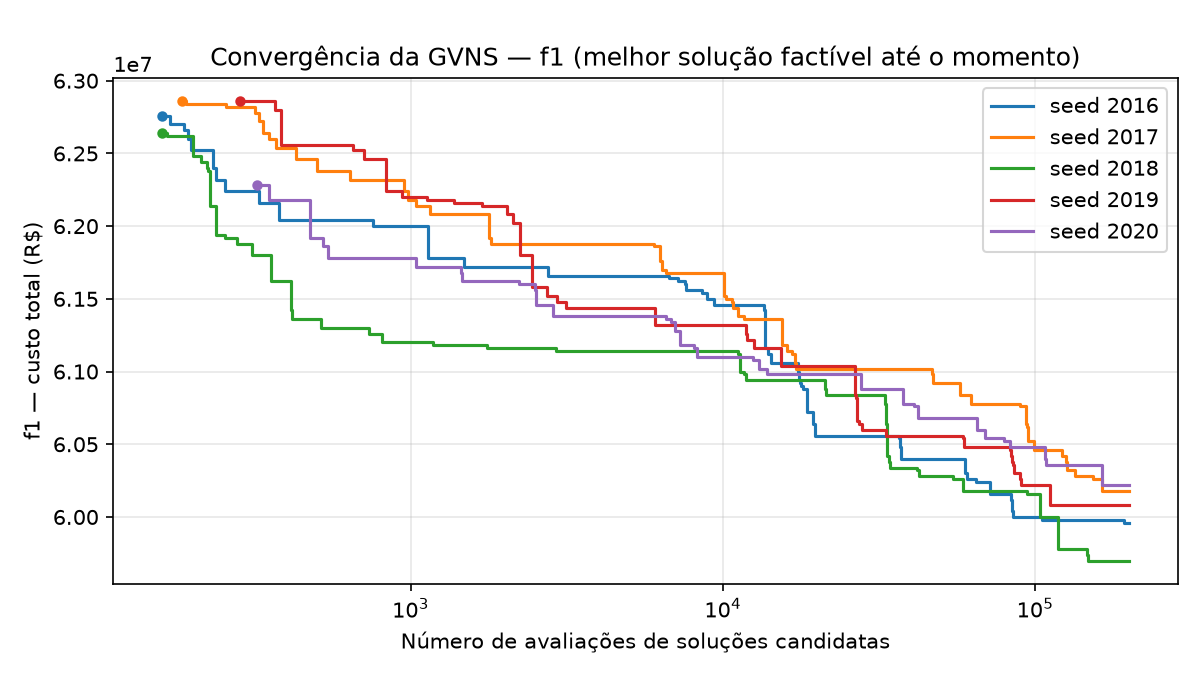
\includegraphics[width=\linewidth]{figures/convergencia_f1.png}\caption{Custo $\fone$.}\end{subfigure}\hfill
\begin{subfigure}[t]{.328\textwidth}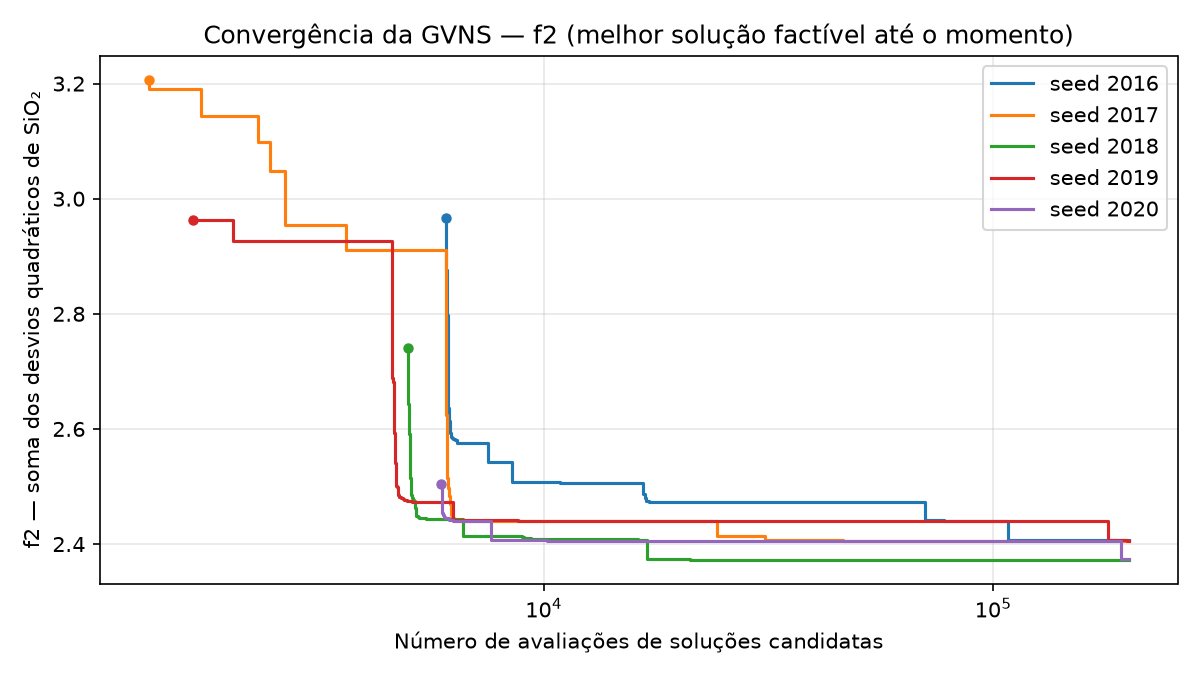
\includegraphics[width=\linewidth]{figures/convergencia_f2.png}\caption{Desvio $\ftwo$.}\end{subfigure}\hfill
\begin{subfigure}[t]{.328\textwidth}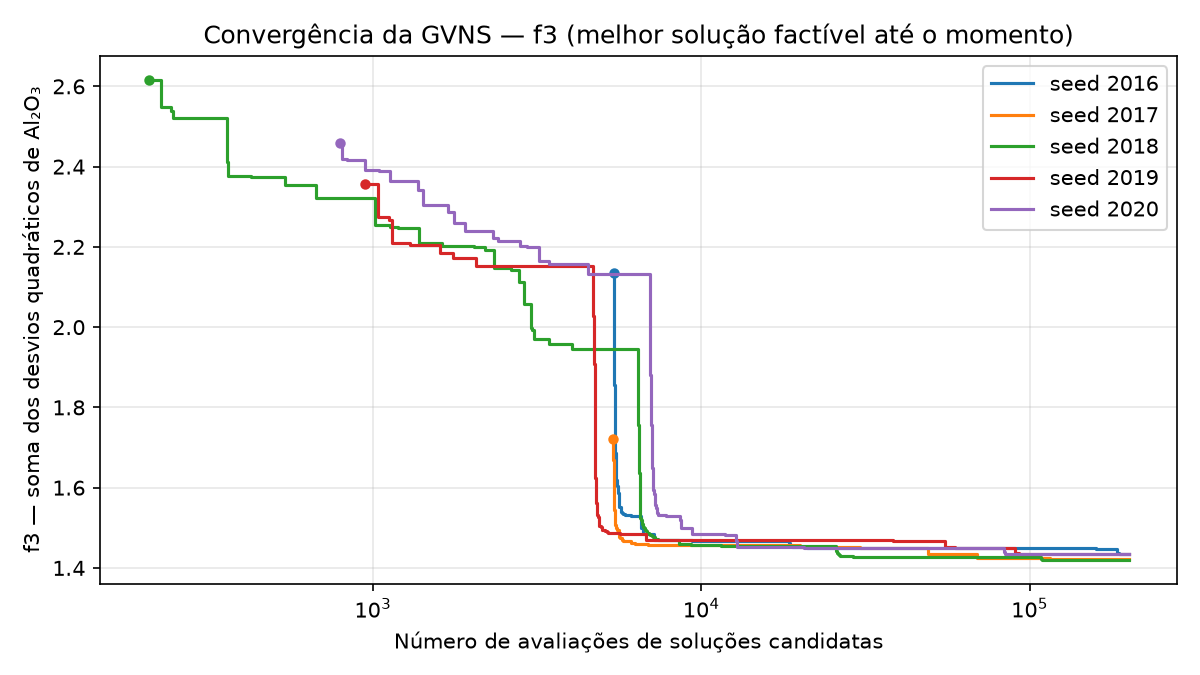
\includegraphics[width=\linewidth]{figures/convergencia_f3.png}\caption{Desvio $\fthree$.}\end{subfigure}
\caption{Curvas de convergência mono-objetivo, com as cinco seeds por critério sobrepostas (2016--2020). Círculos indicam a primeira solução factível; eixos horizontais contam avaliações de candidatos.}\label{fig:conv}
\end{figure*}

\begin{figure*}[!t]
\centering
\begin{subfigure}[t]{.327\textwidth}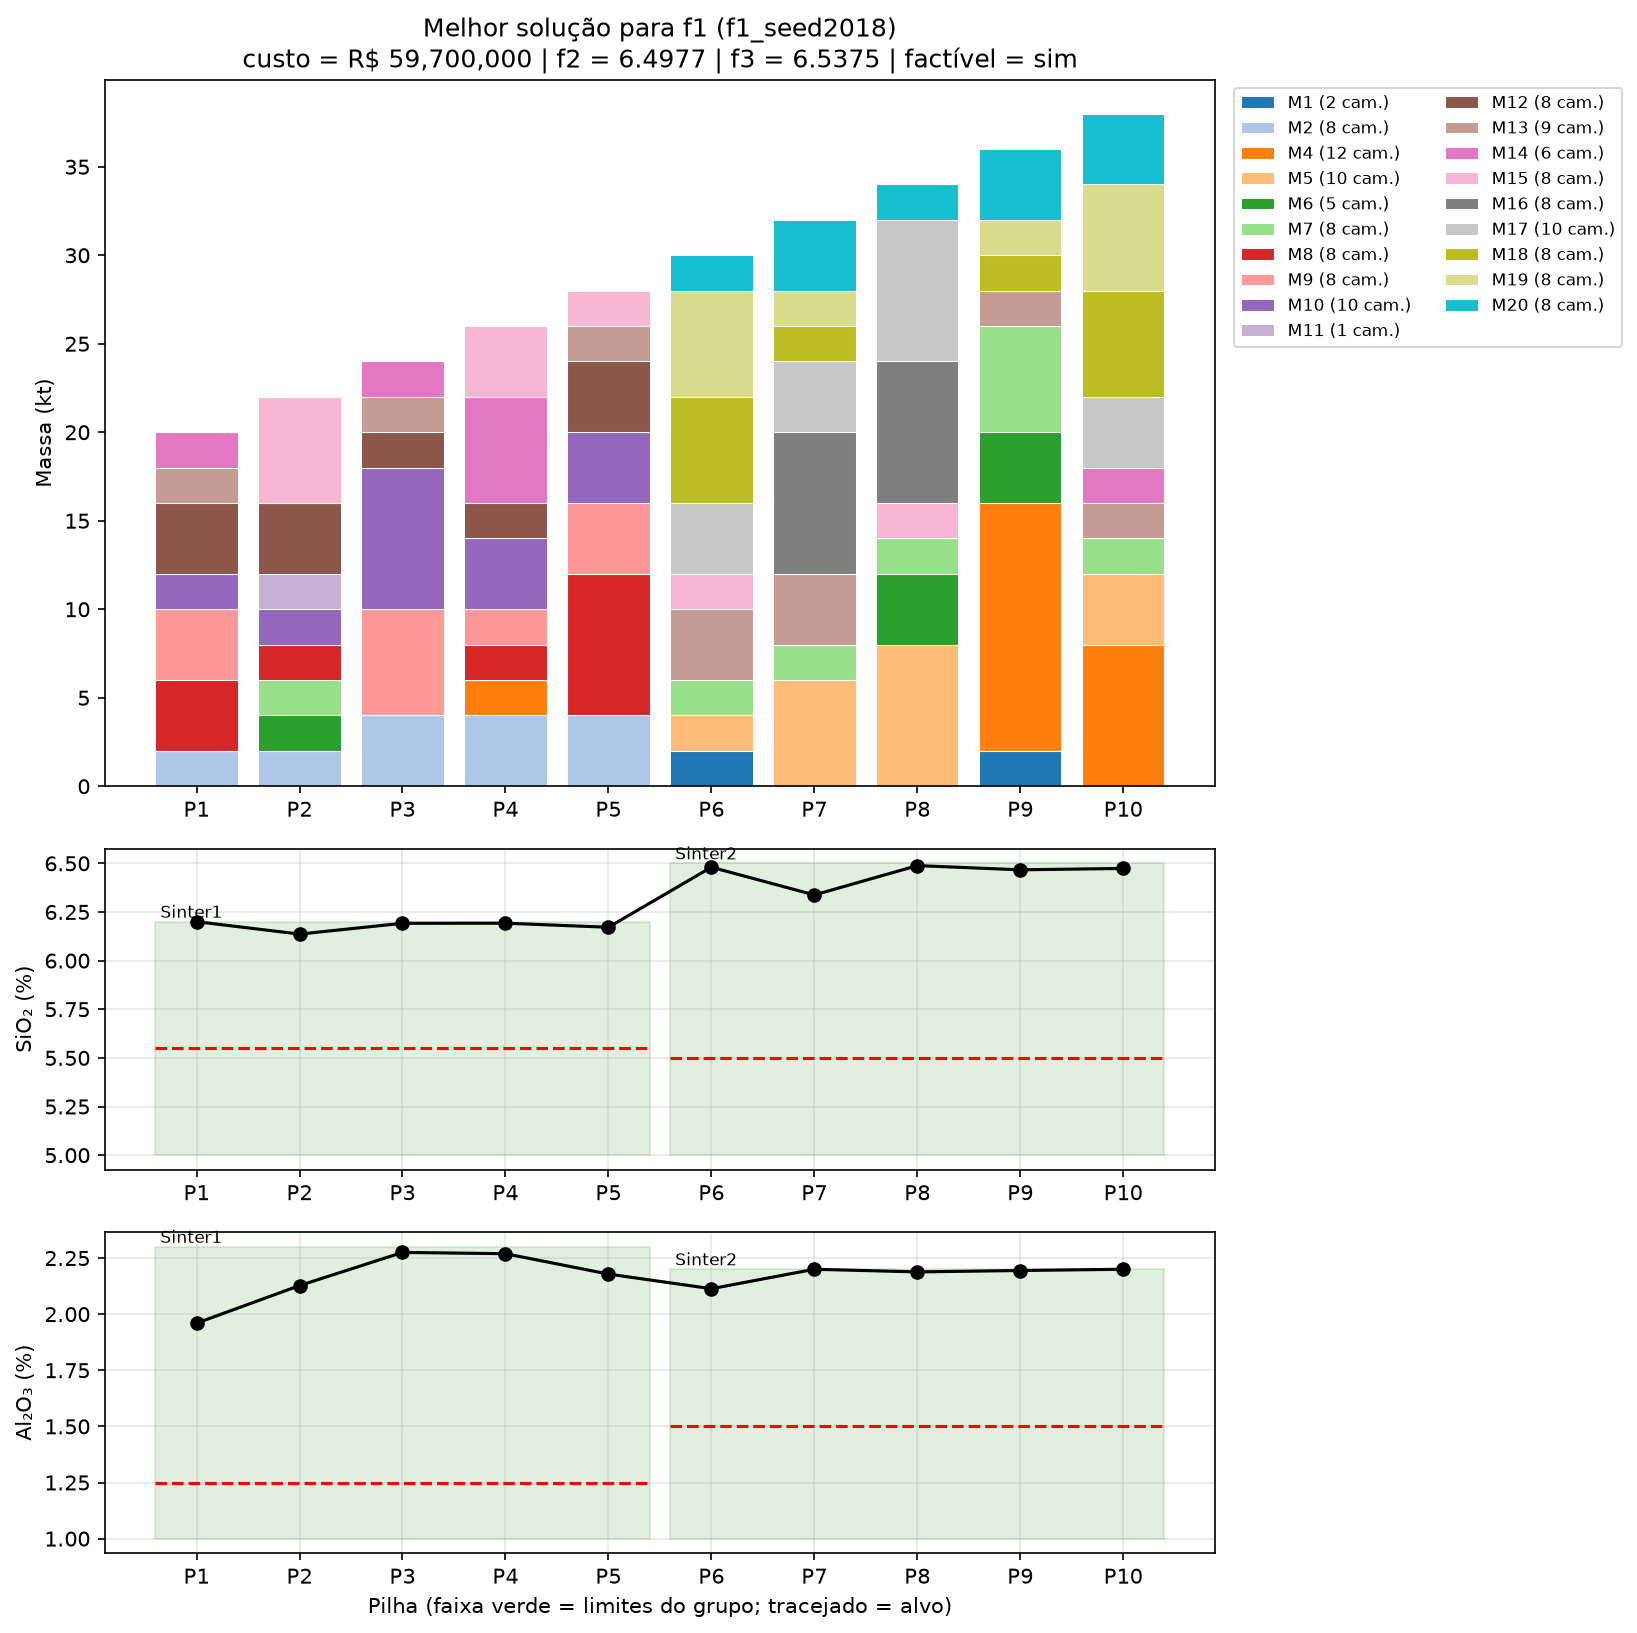
\includegraphics[width=\linewidth]{figures/composicao_f1.png}\caption{Melhor solução de custo.}\end{subfigure}\hfill
\begin{subfigure}[t]{.327\textwidth}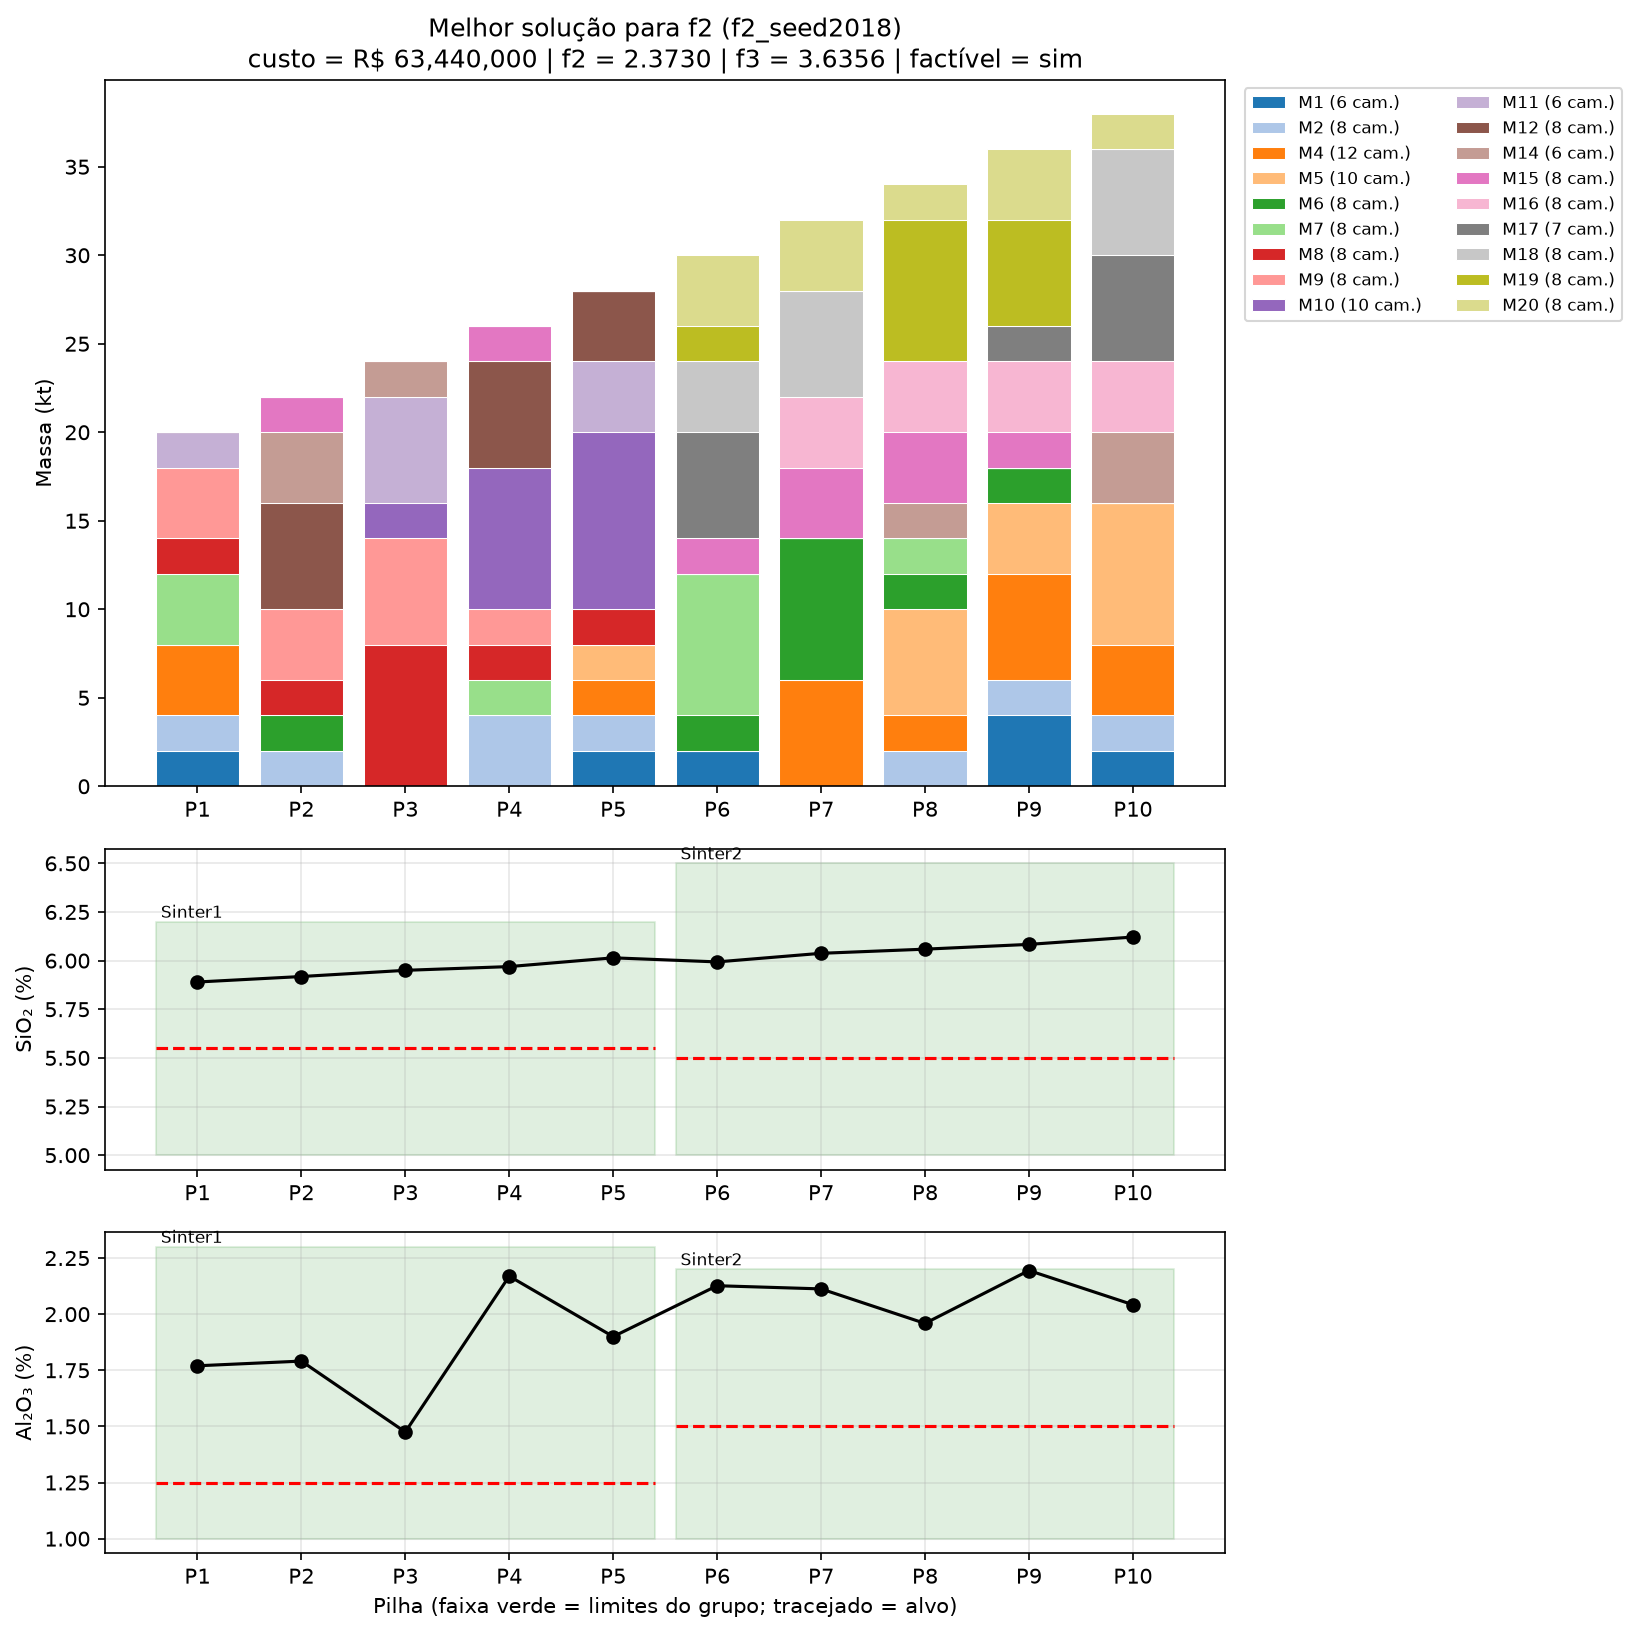
\includegraphics[width=\linewidth]{figures/composicao_f2.png}\caption{Melhor solução de sílica.}\end{subfigure}\hfill
\begin{subfigure}[t]{.327\textwidth}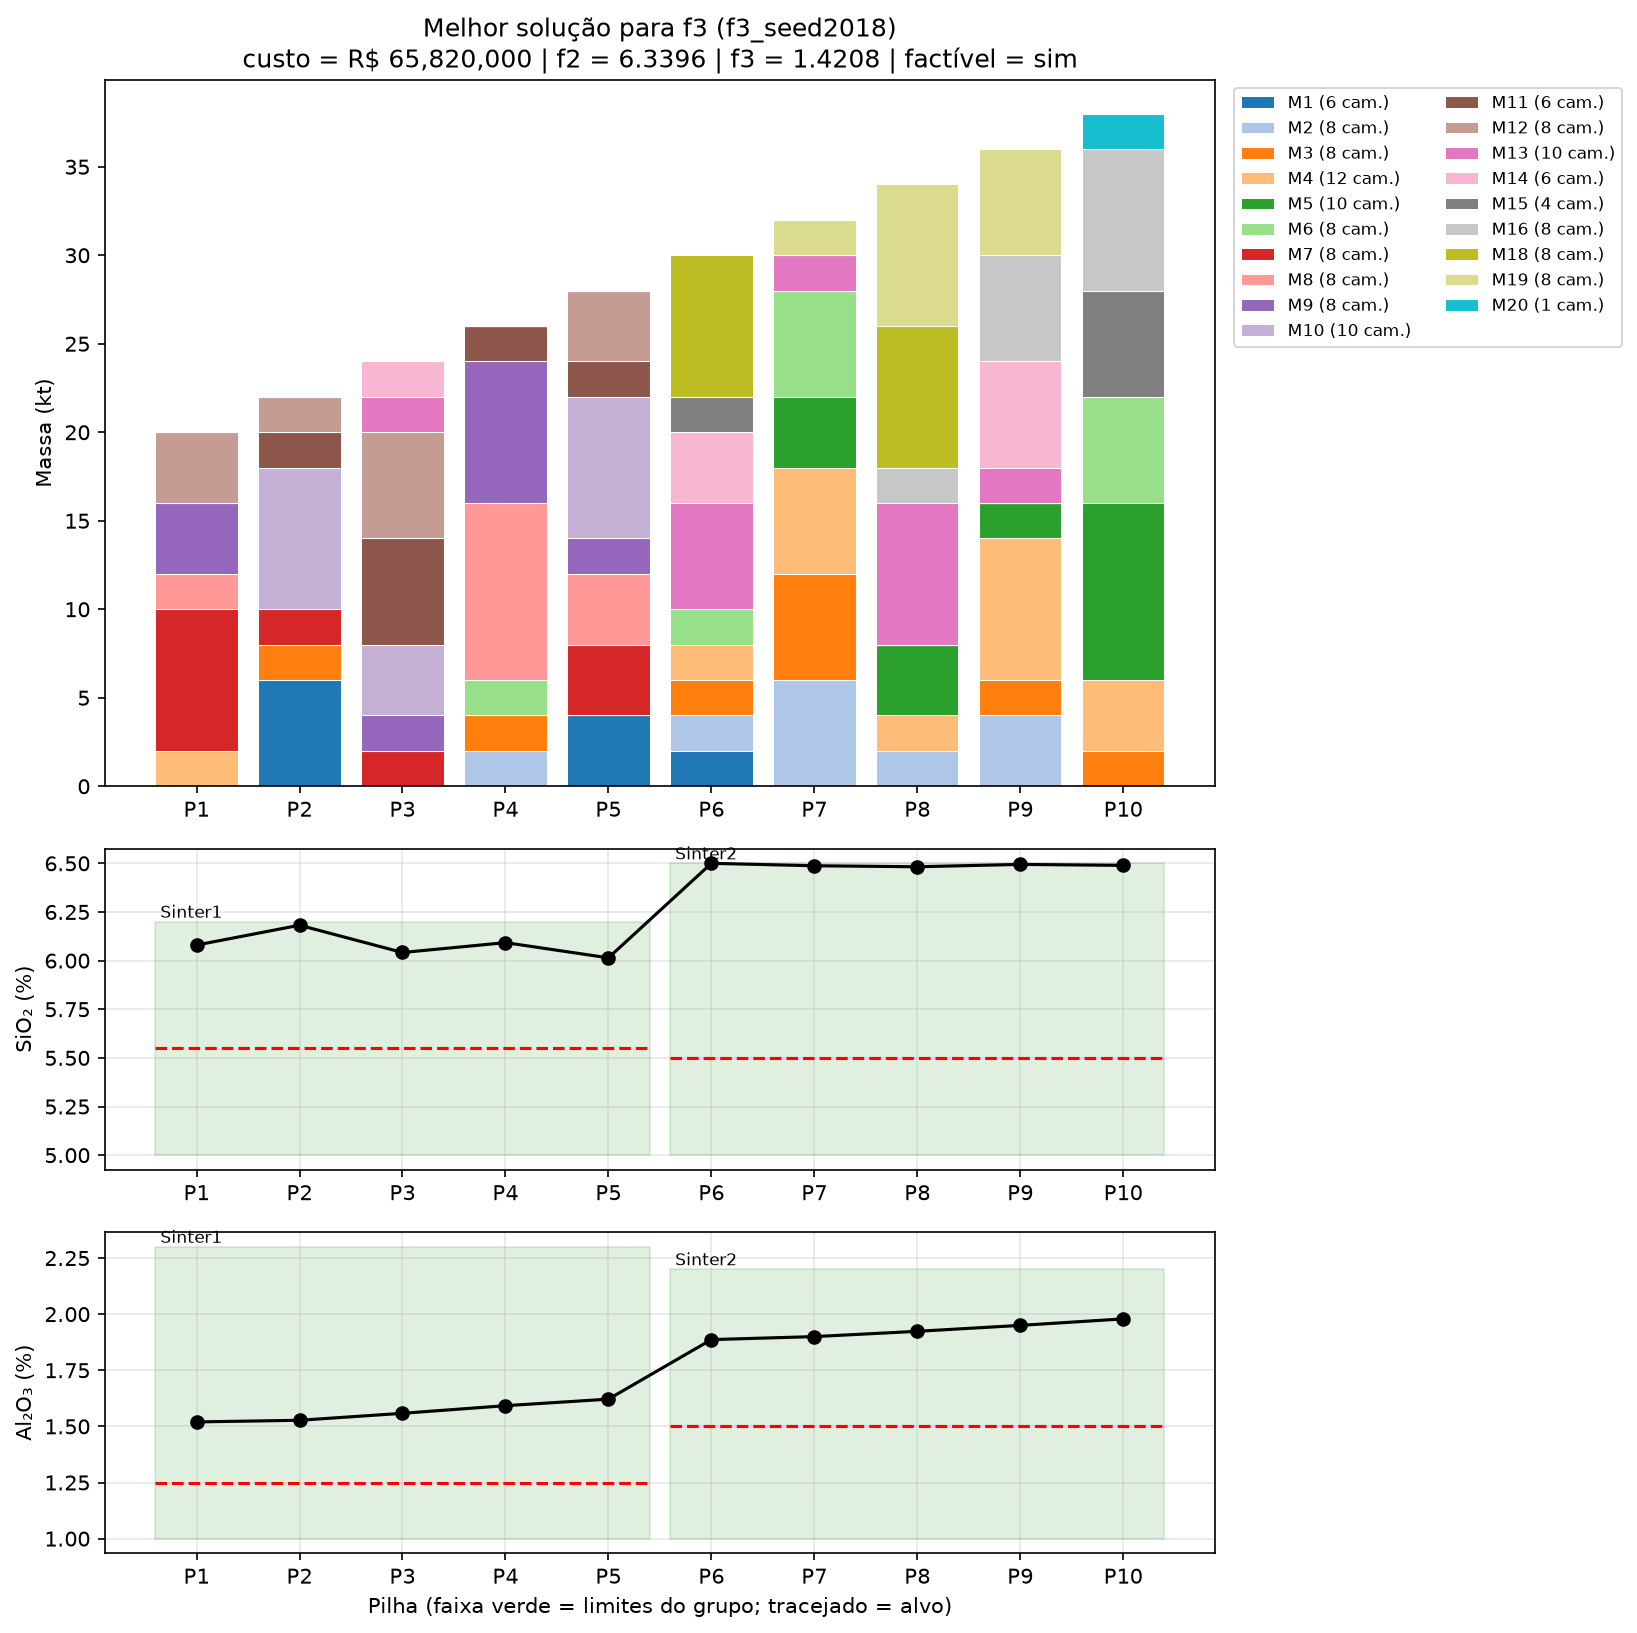
\includegraphics[width=\linewidth]{figures/composicao_f3.png}\caption{Melhor solução de alumina.}\end{subfigure}
\caption{Visualizações das melhores soluções mono-objetivo da seed 2018: composição por minérios e pilhas (parte superior) e teores químicos diante de limites e alvos (parte inferior).}\label{fig:compositions}
\end{figure*}

\subsection{Uso efetivo das vizinhanças}
Os contadores internos da rodada mono-objetivo permitem interpretar a contribuição de cada operador à VND (Tabela~\ref{tab:neigh-stats}). Nas buscas de custo, N2 não produz melhorias estritas após a factibilidade porque preserva a quantidade global de cada minério, e portanto o custo. Ao otimizar desvios químicos, a mesma troca N2 é muito útil, pois redistribui minérios entre pilhas sem alterar disponibilidade global.

\begin{table}[!t]
\centering\caption{Média de melhorias locais produzidas por vizinhança nas cinco execuções de cada versão mono-objetivo.}\label{tab:neigh-stats}
\small\setlength{\tabcolsep}{10pt}
\begin{tabular}{@{}lrrr@{}}\toprule
Objetivo ativo&N1&N2&N3\\\midrule
Custo $\fone$&775,2&0,0&1,6\\
Sílica $\ftwo$&256,0&752,0&0,2\\
Alumina $\fthree$&315,6&995,4&0,0\\\bottomrule
\end{tabular}
\end{table}

A N3 produziu poucas melhorias diretas, mas não é redundante: cada vizinho envolve duas alterações coordenadas, diferentemente da N1, e pode mudar o consumo global, diferentemente da N2. O algoritmo amostra somente 250 movimentos de uma vizinhança potencialmente muito maior; assim, um contador pequeno \textbf{não demonstra que a N3 completa seja inútil}. A diversificação principal permanece responsabilidade do SHAKE, não das vizinhanças locais. As médias de acionamento do SHAKE P1/P2/P3 foram, respectivamente, 19,2/14,0/10,0 em custo, 12,2/9,6/7,8 em sílica e 9,8/7,0/6,2 em alumina.

\section{Formulação multiobjetivo da Entrega 2}
Denote-se por $\mathcal X$ o conjunto admissível definido pelas restrições da Seção 2. O problema vetorial é $\min_{X\in\mathcal X}(\fone(X),\ftwo(X),\fthree(X))$. Uma solução $X$ domina $Y$ quando $f_j(X)\le f_j(Y)$ para os três objetivos e a desigualdade é estrita para pelo menos um deles. As duas escalarizações convertem o problema em famílias de buscas mono-objetivo, reutilizando exatamente a mesma representação e a mesma GVNS (D018--D020).

\subsection{Normalização por referências da Entrega 1}
As unidades do custo (dezenas de milhões de reais) e dos desvios (ordem de unidades) tornam inadequada a agregação direta. Para cada função, usamos os valores das três melhores soluções mono-objetivo factíveis, uma por objetivo, como \textbf{âncoras empíricas}. Definem-se $z_j^*$ como o menor valor de $f_j$ nas âncoras e $z_j^{\mathrm{ref}}$ como o maior. A normalização min--max fixa é
\begin{equation}
 \normal{j}(X)=\frac{f_j(X)-z_j^*}{z_j^{\mathrm{ref}}-z_j^*},\qquad j=1,2,3.
 \label{eq:norm}
\end{equation}

\begin{table}[!t]
\centering\caption{Âncoras da seed 2018 e referências fixas (custo em R\$ mi).}\label{tab:anchors}
\scriptsize\setlength{\tabcolsep}{4pt}
\begin{tabular}{@{}lrrr@{}}\toprule
Solução / referência&$\fone$&$\ftwo$&$\fthree$\\\midrule
$X_1$ (melhor $\fone$)&59,70&6,4977&6,5375\\
$X_2$ (melhor $\ftwo$)&63,44&2,3730&3,6356\\
$X_3$ (melhor $\fthree$)&65,82&6,3396&1,4208\\\midrule
$z^*$ (ideal estimado)&59,70&2,3730&1,4208\\
$z^{\rm ref}$ (referência sup.)&65,82&6,4977&6,5375\\\bottomrule
\end{tabular}
\end{table}

Os valores exatos estão em \texttt{data/referencias\_multiobjetivo.json}; a Tabela~\ref{tab:anchors} usa arredondamento de apresentação. $z^*$ \textbf{não} é um ideal global comprovado e $z^{\mathrm{ref}}$ \textbf{não} é o nadir verdadeiro. Como não se aplica truncamento, $\normal{j}$ pode ser negativo ou maior que 1 quando uma nova solução supera as referências empíricas.

\subsection{Soma Ponderada}
Para cada vetor de pesos fixo $w$, resolve-se
\begin{equation}
 \min_{X\in\mathcal X} F_w(X)=\sum_{j=1}^3 w_j\normal{j}(X),\quad
 w_j\ge0,\quad\sum_{j=1}^3 w_j=1.
 \label{eq:weighted}
\end{equation}
Pesos nulos possibilitam otimizar objetivos isolados ou pares de objetivos. O método pode deixar de recuperar soluções não suportadas da frente eficiente em espaços de objetivos não convexos ou discretos. Por isso, as soluções finais serão sempre submetidas a filtragem de dominância em três dimensões; não presumimos que qualquer resultado escalar seja Pareto-ótimo.

\subsection{Método $\eps$-restrito}
Adotamos o custo normalizado como objetivo principal:
\begin{equation}
 \min_{X\in\mathcal X}\normal{1}(X),\quad
 \normal{2}(X)\le\eps_2,\quad\normal{3}(X)\le\eps_3.
 \label{eq:epsilon}
\end{equation}
As restrições da instância original continuam vigentes. A factibilidade \emph{escalar} também exige ambas as desigualdades de $\eps$; a factibilidade física/química \emph{original} permanece registrada separadamente. Para soluções escalares inviáveis, amplia-se a violação de D007:
\begin{equation}
 V_{\eps}(X)=V(X)+\max\{0,\normal{2}(X)-\eps_2\}
 +\max\{0,\normal{3}(X)-\eps_3\}.
 \label{eq:veps}
\end{equation}
Essa soma é uma regra heurística de comparação, não um certificado de que sempre será encontrada uma solução factível.

\section{Protocolo experimental multiobjetivo}
\subsection{Grades de parâmetros e execução exploratória}
A Soma Ponderada foi investigada por \textbf{16 vetores}: os quinze vetores da malha simplex $w_j=k_j/4$, com $k_j\in\{0,1,2,3,4\}$ e $\sum k_j=4$, acrescidos de $(1/3,1/3,1/3)$. A grade inclui vértices, combinações entre dois objetivos e o compromisso central.

No $\eps$-restrito, foi utilizado o produto cartesiano $\eps_2,\eps_3\in\{0,25;\,0,50;\,0,75;\,1,00\}$, também com \textbf{16 configurações}. A grade completa, ao contrário de uma variação apenas na diagonal, permite controlar cada desvio químico separadamente. A Tabela~\ref{tab:eps} traduz cada nível em limite na escala original, por $f_j\le z_j^*+\eps_j(z_j^{\rm ref}-z_j^*)$.

\begin{table}[!t]
\centering\caption{Correspondência dos limites $\eps$ na escala dos desvios quadráticos originais.}\label{tab:eps}
\small\setlength{\tabcolsep}{11pt}
\begin{tabular}{@{}rrr@{}}\toprule
$\eps$&Limite $\ftwo$&Limite $\fthree$\\\midrule
0,25&3,4042&2,6999\\
0,50&4,4354&3,9791\\
0,75&5,4665&5,2583\\
1,00&6,4977&6,5375\\\bottomrule
\end{tabular}
\end{table}

O planejamento (D021) separou as seeds exploratórias 4001 e 4002 das seeds oficiais. Foram executadas as 32 configurações com budgets de 50k, 100k e 200k avaliações e ambas as seeds: todas as 64 execuções por orçamento terminaram factíveis. Ao passar de 100k para 200k, \textbf{27 das 32 execuções de cada método melhoraram o objetivo escalar}, sem piora das demais. As inversões de monotonicidade heurística do custo entre pares aninhados de limites $\eps$ caíram de 7 para 4 e 2, respectivamente, entre 50k, 100k e 200k (mesmas duas seeds).

\subsection{Rodada oficial congelada e filtro Pareto}
Após o piloto, os parâmetros foram congelados no commit anterior às execuções (D021--D022): cinco seeds \textbf{2021--2025}, 200.000 avaliações por execução, \texttt{sample\_size}=250 e SHAKE P1/P2/P3 = 3/4/5. São $16\times5=80$ execuções por abordagem, \textbf{160 execuções e 32 milhões de avaliações} no total, com a mesma medida de esforço por método. Os resultados oficiais pertencem à versão de código \texttt{d5e0d94}.

Para cada abordagem, reúnem-se apenas as \emph{melhores soluções finais escalares factíveis} de todas as configurações e seeds. A dominância é testada nos \textbf{três objetivos originais} $(\fone,\ftwo,\fthree)$, e só então os pontos são projetados nos pares $\fone\times\ftwo$, $\fone\times\fthree$ e $\ftwo\times\fthree$. Um ponto não dominado no espaço 3D pode parecer dominado numa projeção 2D; o filtro não é repetido separadamente na projeção. Vetores coincidentes são unificados nas figuras, preservando-se IDs de origem nos CSVs. As frentes são \emph{empíricas}, não a fronteira Pareto global certificada.

\section{Resultados oficiais multiobjetivo}
\subsection{Validade, cobertura e extremos}
As 160 execuções terminaram factíveis tanto no problema original quanto na respectiva escalarização, e atingiram exatamente o orçamento. A verificação dos registros indicou consistência entre objetivos originais/normalizados, pesos, limites $\eps$ e valor escalar. A Soma Ponderada gerou \textbf{45 vetores não dominados distintos}; o $\eps$-restrito, \textbf{49}. Na união, \textbf{91 vetores distintos} permanecem não dominados: 44 originados da Soma Ponderada e 47 do $\eps$-restrito. Apenas um vetor da frente de Soma Ponderada é dominado por alguma solução da outra abordagem e dois do $\eps$-restrito são dominados por resultados de Soma Ponderada.

\begin{table*}[!t]
\centering\caption{Resultados oficiais da Entrega 2 por abordagem. Os extremos de colunas distintas podem pertencer a soluções diferentes.}\label{tab:multi-result}
\footnotesize\setlength{\tabcolsep}{5pt}
\begin{tabular}{@{}lcccccc@{}}\toprule
Método&Execuções factíveis&Vetores próprios&Na frente conjunta&Custo $\fone$ (R\$ mi)&$\ftwo$&$\fthree$\\\midrule
Soma Ponderada&80/80&45&44&59,68--65,82&2,3728--6,9396&1,4215--6,6346\\
$\eps$-restrito&80/80&49&47&59,86--63,74&3,3672--6,4940&2,6698--6,1604\\\midrule
\multicolumn{3}{@{}l}{Frente não dominada conjunta} &\textbf{91}&&&\\\bottomrule
\end{tabular}
\end{table*}

O menor custo foi encontrado em \texttt{w15/2021}: $\fone=\mathrm{R}\$\,59,68$ milhões, $\ftwo=6,88569$ e $\fthree=6,63457$. O menor $\ftwo$ ocorreu em \texttt{w05/2022}, $\ftwo=2,372752$ e custo de R\$ 63,44 milhões, isto é, 6,30\% mais caro que a solução anterior, mas com 65,5\% menos desvio de sílica. O menor $\fthree$ ocorreu em \texttt{w01/2022}, $\fthree=1,421458$ e custo de R\$ 65,82 milhões: cerca de 10,3\% mais caro e 78,6\% menos desvio de alumina. Trata-se de comparações entre soluções observadas, não de garantias de compromisso ótimo.

\subsection{Cobertura da Soma Ponderada}
A Soma Ponderada recuperou os extremos e apresentou agrupamentos separados no espaço de qualidade. Com $w=(0,1,0)$, aproximou-se do melhor desvio de sílica mono-objetivo; com $w=(1,0,0)$, encontrou custo menor que a própria âncora empírica, produzindo $\normal{1}\simeq-0,00327$. A escala não foi truncada, como previsto em D018.

Os pesos \texttt{w02}, \texttt{w03} e \texttt{w07} produziram soluções muito semelhantes ($\fone\simeq\mathrm{R}\$\,65,46$ milhões; $\ftwo\simeq2,68$; $\fthree\simeq1,69$), ilustrando \emph{redundância de pesos}. Na frente própria, nenhuma solução da Soma Ponderada tem $2,90<\ftwo<5,44$, enquanto o $\eps$-restrito possui \textbf{32 vetores não dominados próprios} nesse intervalo, como conferido nos CSVs oficiais. A ausência de cobertura intermediária é compatível com a limitação das somas ponderadas em regiões não suportadas, embora também dependa da grade e da própria GVNS.

\subsection{Cobertura e interpretação do $\eps$-restrito}
Os resultados se organizam próximos às fronteiras de desvio introduzidas pela grade. Na configuração $\texttt{e01}=(0,25;0,25)$, a média de custo das cinco seeds foi R\$ 63,732 milhões; na configuração $\texttt{e16}=(1;1)$, R\$ 60,052 milhões, uma redução de \textbf{R\$ 3,680 milhões} (5,8\%) à custa de maiores desvios químicos. Nas configurações diagonais intermediárias, e06=(0,50;0,50) e e11=(0,75;0,75), os custos médios foram R\$ 62,104 e R\$ 60,836 milhões, respectivamente.

Como o nível mínimo testado foi 0,25, a abordagem não amostrou regiões próximas de $\normal{2}=0$ ou $\normal{3}=0$. Essa é uma \textbf{limitação da grade}, não uma impossibilidade do método. Da mesma forma, $\eps_2=\eps_3=1$ não remove as restrições: 14 das 80 soluções finais da Soma Ponderada possuem pelo menos um objetivo químico normalizado acima de 1. A solução mais barata observada, por exemplo, tem $\normal{2}=1,09406$ e $\normal{3}=1,01897$ e não pertence ao domínio factível de e16.

A monotonicidade do \emph{ótimo global} exige que relaxar limites não aumente o menor custo factível. Na rodada oficial houve somente \textbf{três inversões em 420 comparações} de pares aninhados dentro da mesma seed, todas pequenas (maior diferença R\$ 260 mil). São falhas de monotonicidade das \emph{melhores soluções heurísticas encontradas}, não da formulação. Nas médias das cinco seeds, a única inversão entre pares aninhados foi e07$\to$e08, um aumento de R\$ 84 mil apesar do relaxamento de $\eps_3$.

\subsection{Variabilidade das cinco sementes}
Todas as seeds contribuíram com vetores não dominados. Na ordem 2021--2025, as contribuições às frentes \emph{próprias} foram 7, 11, 8, 10 e 9 para Soma Ponderada; 8, 11, 10, 10 e 10 para $\eps$-restrito. Não houve uma seed isolada responsável pela maior parte da cobertura.

Para medir a dispersão dentro de cada configuração, calculou-se o desvio-padrão \emph{amostral} das cinco execuções e, depois, a \textbf{mediana dos 16 desvios-padrão por método}. Para custo, as medianas foram \textbf{R\$ 44,5 mil} (Soma Ponderada) e \textbf{R\$ 91,0 mil} ($\eps$-restrito); para $\ftwo$, 0,0188 e 0,0204; para $\fthree$, 0,1025 e 0,0261, respectivamente. São descrições da variabilidade \emph{condicionada às grades escolhidas}, não um teste de superioridade estatística.

Sete das 16 configurações de peso apresentaram o mesmo custo final nas cinco seeds, embora os objetivos químicos possam variar. Em \texttt{w15}, a amplitude do custo atingiu R\$ 660 mil. No $\eps$-restrito, a amplitude máxima foi R\$ 540 mil, em \texttt{e12}. Na configuração permissiva e16, o desvio-padrão de $\fthree$ foi aproximadamente 0,464: mesmo com limite químico não ativo para algumas soluções, a composição pode variar entre mínimos de custo semelhantes.

A cobertura visual e o número de contribuições mostram que as execuções alcançaram regiões semelhantes em termos gerais, mas não necessariamente o mesmo vetor, especialmente nos objetivos pouco priorizados. A comparação de médias globais de custo entre métodos deve ser evitada como ranking: as grades exploram regiões factíveis diferentes.

\subsection{Projeções bidimensionais das frentes}
A Fig.~\ref{fig:pareto} dispõe cada projeção lado a lado para comparação direta. As cores identificam as sementes; quando diferentes configurações produzem objetivos coincidentes, as origens completas permanecem nos arquivos \texttt{pareto\_*.csv}. A Soma Ponderada concentra pontos nos extremos, enquanto o $\eps$-restrito distribui soluções em faixas ligadas aos limites químicos, sobretudo na região intermediária.

\clearpage
\onecolumn
\begin{figure}[p]
\centering
\small\textbf{Soma Ponderada}\hspace{.36\textwidth}\textbf{$\eps$-restrito}\par\vspace{4pt}
\begin{tabular}{@{}cc@{}}
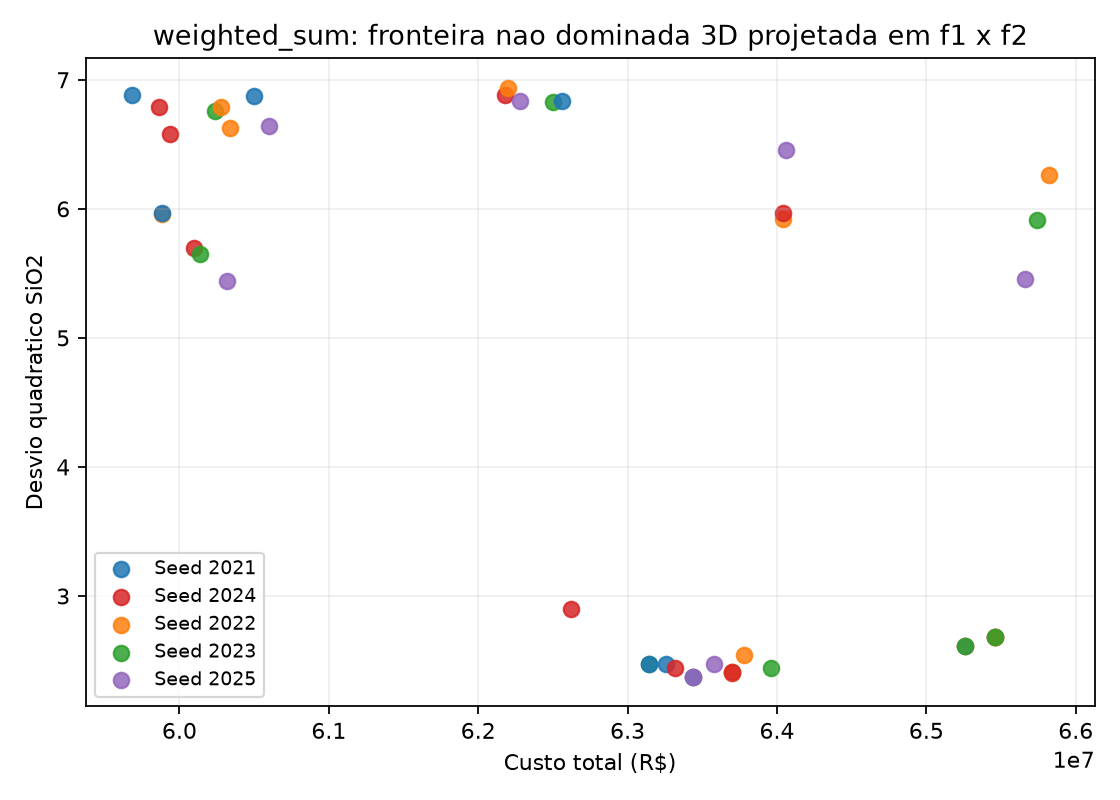
\includegraphics[width=.48\textwidth]{figures/soma_f1_f2.png} & 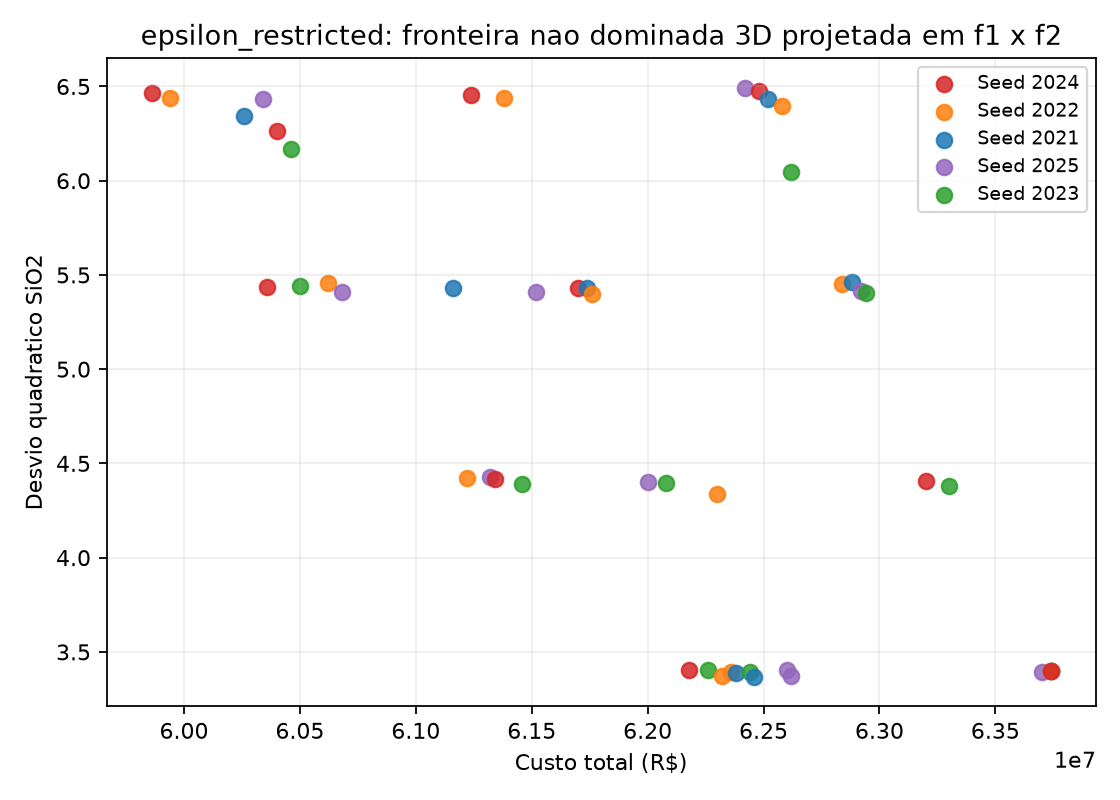
\includegraphics[width=.48\textwidth]{figures/epsilon_f1_f2.png}\\[-2pt]
\multicolumn{2}{c}{\small (a) Projeção $\fone\times\ftwo$: custo e desvio de \Si.}\\[3pt]
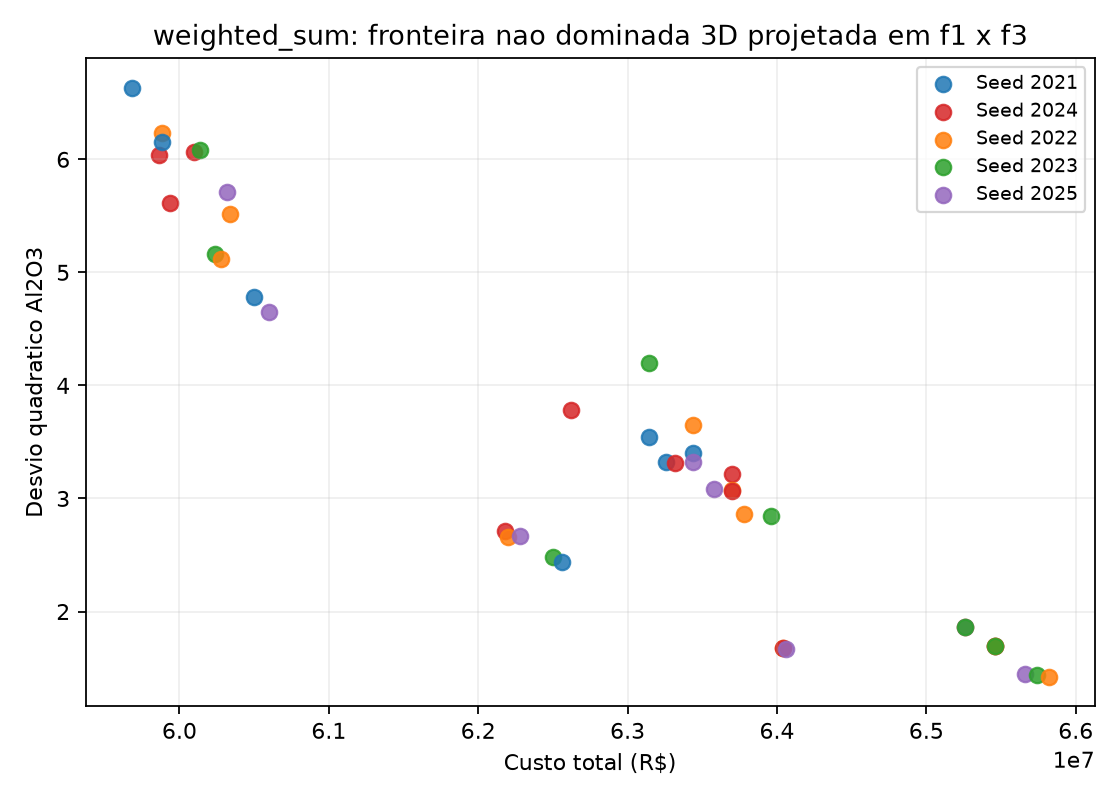
\includegraphics[width=.48\textwidth]{figures/soma_f1_f3.png} & 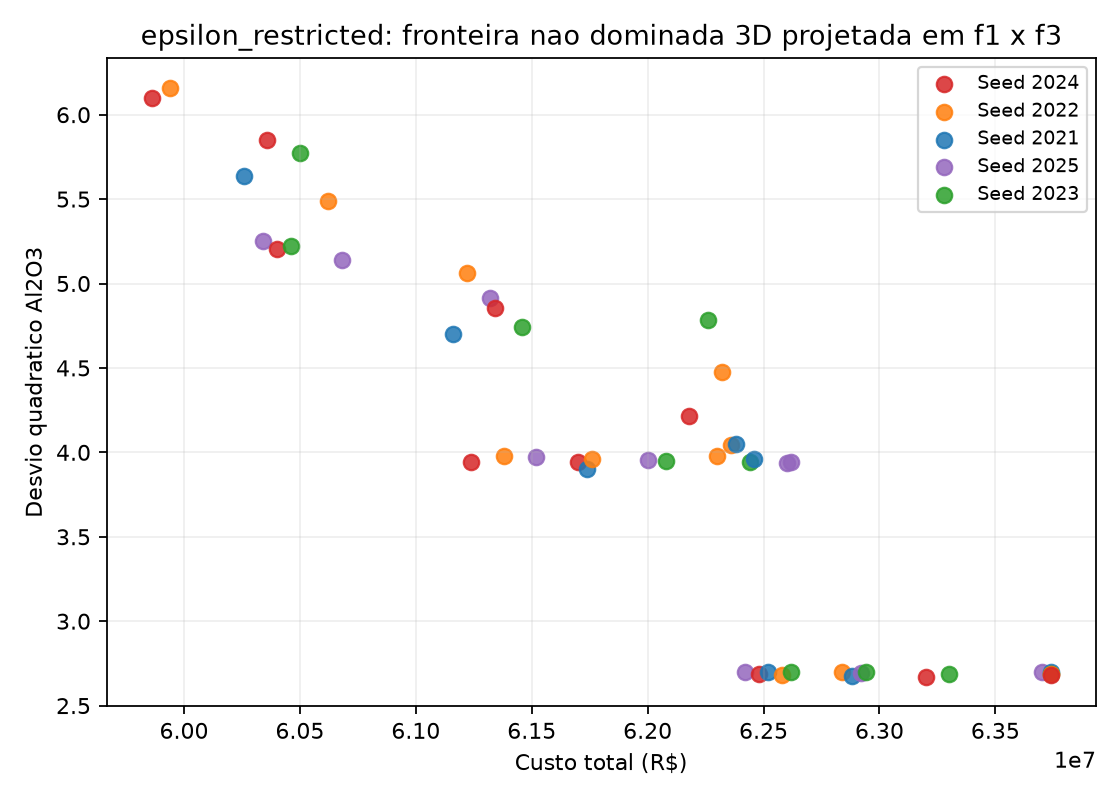
\includegraphics[width=.48\textwidth]{figures/epsilon_f1_f3.png}\\[-2pt]
\multicolumn{2}{c}{\small (b) Projeção $\fone\times\fthree$: custo e desvio de \Al.}\\[3pt]
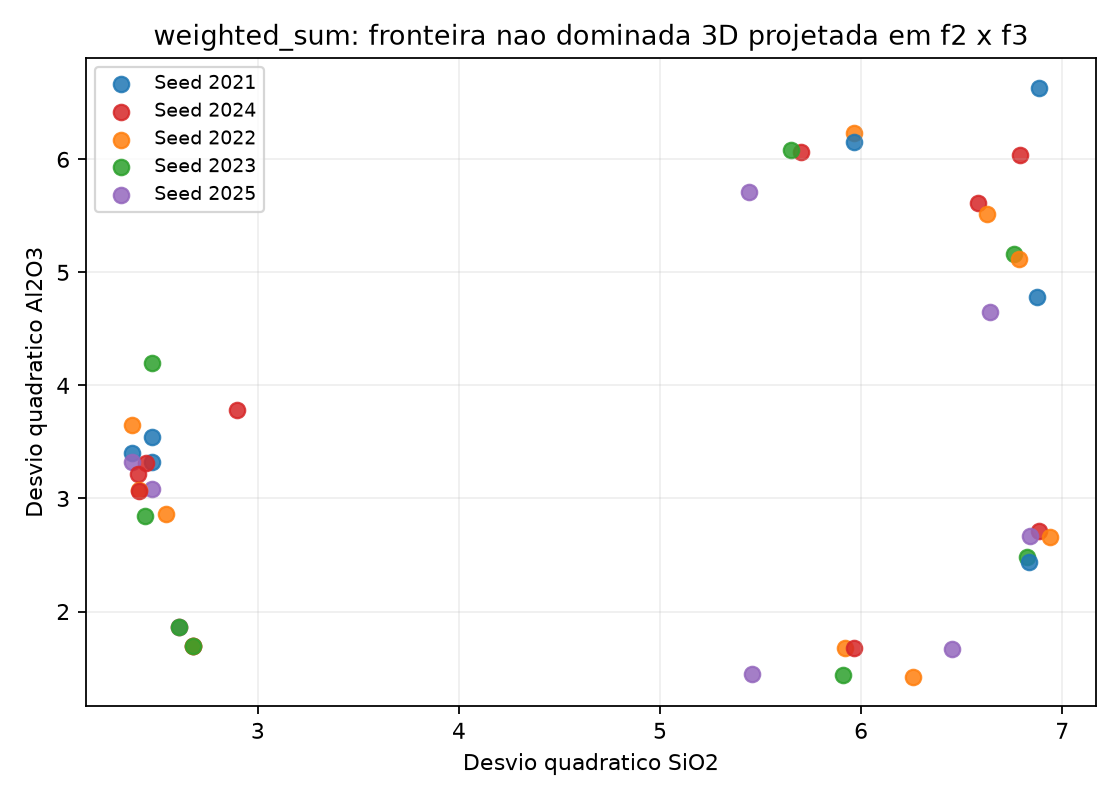
\includegraphics[width=.48\textwidth]{figures/soma_f2_f3.png} & 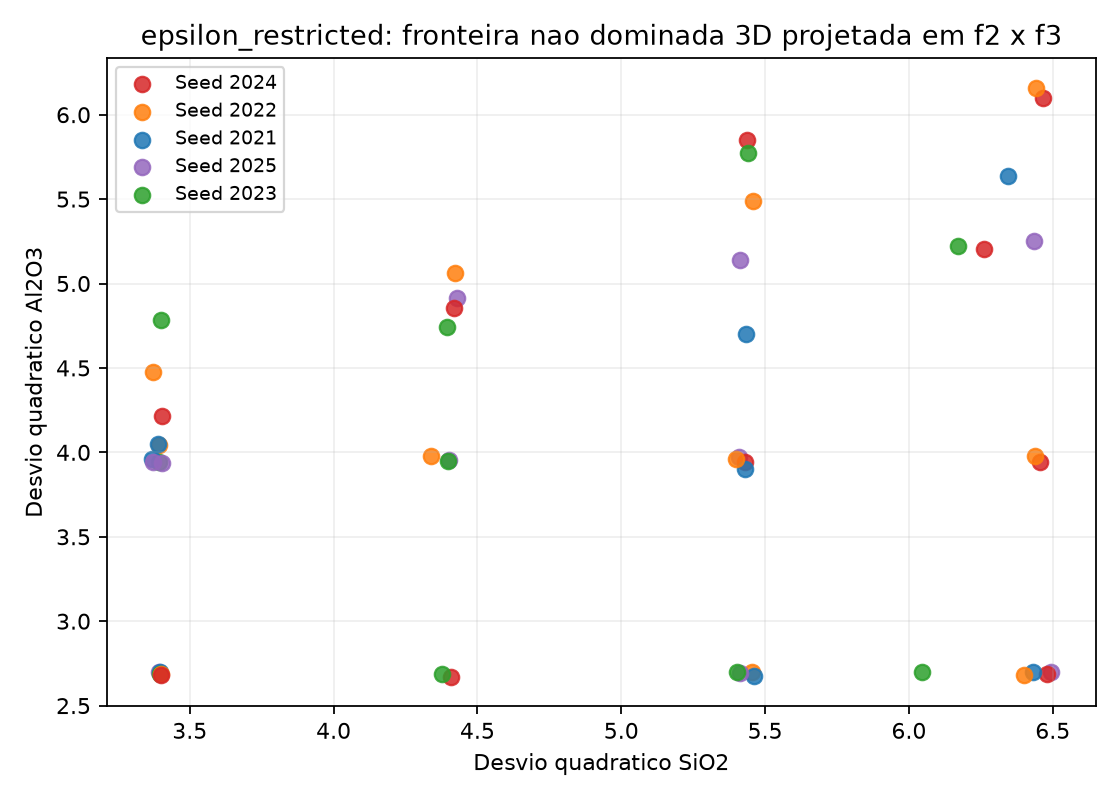
\includegraphics[width=.48\textwidth]{figures/epsilon_f2_f3.png}\\[-2pt]
\multicolumn{2}{c}{\small (c) Projeção $\ftwo\times\fthree$: desvios químicos.}\\
\end{tabular}
\caption{Seis projeções das frentes não dominadas em três objetivos, comparadas lado a lado. As cores identificam as seeds 2021--2025. Os pontos foram filtrados em três dimensões, não novamente em cada projeção.}\label{fig:pareto}
\end{figure}
\clearpage
\twocolumn

\section{Reprodutibilidade e limitações}
Os resultados oficiais estão em \texttt{results/multi\_final/}: 160 arquivos JSON de execução, \texttt{summary.csv}, estatísticas por configuração, CSVs das frentes, seis figuras e \texttt{manifest.json}. Este último registra \texttt{git\_version=d5e0d94} e protocolo \texttt{CONGELADO}; a execução exigiu cinco sementes fixas e orçamento idêntico para as duas abordagens.

A execução multiobjetivo é descrita em \texttt{docs/entrega2\_experimentos.md} e pode ser iniciada, em um checkout consistente com a versão histórica, por:
\begin{lstlisting}[style=pseudo]
python -m pip install -e '.[dev]'
python -m pytest -q
python scripts/run_multi_experiments.py --phase final --dry-run
python scripts/run_multi_experiments.py --phase final --out results/multi_repro
\end{lstlisting}
O último comando requer o protocolo já congelado e salva em pasta separada; \textbf{não deve sobrescrever o registro histórico}. A atualização proposta no PR \#4 altera a assinatura dos arquivos para considerar os conteúdos de instância e código; resultados antigos têm assinatura diferente e devem permanecer imutáveis. Esse aperfeiçoamento de auditoria \emph{não foi utilizado} na execução oficial da versão \texttt{d5e0d94}.

Quatro limites de interpretação permanecem: (i) trata-se de uma instância de exemplo; (ii) não há certificação de ótimo global nem de Pareto global; (iii) a grade de pesos e de limites $\eps$ afeta a cobertura; (iv) o arquivo de frentes é construído a partir das melhores soluções finais escalares, não de um arquivo acumulativo de todos os vizinhos encontrados. A Entrega 3 poderá empregar os vetores não dominados obtidos como alternativas para a etapa de decisão multicritério, sem tratar a frente estimada como completa.

\section{Conclusões}
A representação por caminhões, a heurística construtiva e a regra de viabilidade permitiram executar a mesma GVNS nas três versões mono-objetivo e nas duas escalarizações multiobjetivo. A VND combina N1 exaustiva e N2/N3 amostradas; o SHAKE P1/P2/P3 fornece diversificação. A N3 é um movimento atômico de duas substituições articuladas, que altera a composição global sem ser uma troca simples, e sua amostragem por prefixos ponderados é uniforme sobre movimentos distintos.

O orçamento de 200.000 avaliações foi consolidado após pilotos e reproduzido nas 160 execuções finais. Todas foram factíveis. Entre os resultados não dominados, a Soma Ponderada atingiu extremos de custo e qualidade e apresentou lacunas de cobertura; o $\eps$-restrito preencheu boa parte dessas regiões intermediárias, oferecendo limites químicos diretamente interpretáveis. A frente conjunta contém 91 alternativas empíricas, 44 da Soma Ponderada e 47 do $\eps$-restrito. A escolha final de uma composição, envolvendo preferências e atributos adicionais, fica para a Entrega 3.

\begin{thebibliography}{9}\small
\bibitem{case} Universidade Federal de Minas Gerais. \emph{Teoria da Decisão -- Case: Otimização do Custo e Qualidade de Pilhas de Minério}. Enunciado da disciplina, 2026/2.
\bibitem{aula} Universidade Federal de Minas Gerais. \emph{Material de aula de Teoria da Decisão: VNS/GVNS, tratamento de restrições, Soma Ponderada e $\eps$-restrito}. 2026/2.
\bibitem{repo} Grupo do projeto. \emph{cassotis\_optimization}: código, protocolos, decisões e resultados oficiais. \url{https://github.com/peddrinn/cassotis_optimization}. Acesso em 18 out. 2026.
\end{thebibliography}
\end{document}
